% !TEX spellcheck = English (aspell)

\documentclass[a4paper]{article}
\usepackage[utf8]{inputenc}
\usepackage[T1]{fontenc}      
\usepackage[english]{babel} %utilisation du package français
%
\usepackage{textcomp}% améliore certains symboles de bases
\usepackage{lmodern}% remplace la police ComputerModern par LatinModern (+ mieux bien)
%
%\usepackage[a4paper]{geometry} % Pour avoir les marges pour du papier A4
%
%\usepackage[intlimits, leqno]{amsmath}% ams-mathh ! avec numérotation des équations à gauche et intégrales avec limites dessous
\usepackage{mathtools}% compléments à amsmath
\usepackage{amssymb,amsfonts}% symboles mathématiques supplémentaires
%\usepackage{bm}% symbole math gras
\usepackage{amsthm}% environnement ams-theorem
%\usepackage{array}% ajoute des options aux environnements tabular et arrray, permet de centrer
%\usepackage{mathrsfs}% permet d'utiliser matcal
\usepackage[colorlinks,breaklinks,bookmarks,plainpages=false,unicode=true]{hyperref}%
\usepackage{todonotes} %ajouter des commentaires
%\usepackage[disable]{todonotes}%cache les commentaires
\usepackage{datetime} %ajoute la date et l'heure
%\usepackage{here} % permet d'utilser H, h pour place les figures
%
%
\usepackage{tikz}
\usetikzlibrary{external}
\tikzexternalize[prefix=Images/]% On externalise. Les images sont stockées dans le dossier Images
\makeatletter %pour ne pas prendre en compte les todo dans l'externalisation
\renewcommand{\todo}[2][]{\tikzexternaldisable\@todo[#1]{#2}\tikzexternalenable}
\makeatother
\makeatletter %pour ne pas prendre en compte les missingfigures dans l'externalisation
\renewcommand{\missingfigure}[2][]{\tikzexternaldisable\@missingfigure[#1]{#2}\tikzexternalenable}
\makeatother

\tikzset{myloop above/.style={loop, out=130, in = 50,min distance =8mm}}
\tikzset{blacknode/.style={shape= circle, fill = black, inner sep = 0pt, outer sep = 0pt, minimum size = 3pt,draw}}
%
\newtheorem{lem}{Lemma}[section]
%\newtheorem{AFaire}[lemma]{A faire}% peut enlever à la fin
%\newtheorem{Next}[lemma]{Possible continuation}% peut enlever à la fin
\newtheorem{conjecture}[lem]{Conjecture}
\newtheorem{cor}[lem]{Corollary}
\newtheorem{prop}[lem]{Proposition}
%\newtheorem{question}[lem]{Question}
\newtheorem{thm}[lem]{Theorem}
\theoremstyle{definition}
\newtheorem{defn}[lem]{Definition}
\theoremstyle{remark}% texte en roman
%\newtheorem{claim}[lem]{Affirmation}
\newtheorem{exmp}[lem]{Example}
%\newtheorem{fact}[lem]{Fact}
%\newtheorem{notation}[lem]{Notation}
%\newtheorem{rem}[lem]{Remark}
%\newtheorem{scholion}[lem]{Scholion}
%\newtheorem{exo}{Exercise}
%
%
%
\DeclareMathOperator\Cayley{Cayl}
\DeclareMathOperator\Sch{Sch}
\DeclareMathOperator\stab{Stab}
%\DeclareMathOperator\Aut{Aut} 
%\DeclareMathOperator\cl{Cl}
%\DeclareMathOperator\fix{Fix}
%\DeclareMathOperator\GL{GL}		%groupe linéaire
%\DeclareMathOperator\im{im}
%\DeclareMathOperator\id{Id}
%\DeclareMathOperator\Ind{Ind}
%\DeclareMathOperator\orbite{O}
%\DeclareMathOperator\ppcm{ppcm}
%\DeclareMathOperator\pgcd{pgcd}
%\DeclareMathOperator\sign{sign}
%\DeclareMathOperator\SL{SL}		
%\DeclareMathOperator\supp{supp}
%
\DeclarePairedDelimiter\abs{\lvert}{\rvert}
%\DeclarePairedDelimiter\gen{\langle}{\rangle}
%
%\newcommand*{\actsGroup}{\curvearrowright}% sementic command for G acts X
%\newcommand*{\iso}{\cong}% isomorphisme,commande sémantique (\simeq ou \cong)
%\renewcommand*{\H}{\mathcal{H}}
%\renewcommand*{\S}{\mathcal{S}}

\newcommand*{\field}[1]{\mathbf{#1}}
%\newcommand*{\N}{\field{N}}
\newcommand*{\Z}{\field{Z}}
%\newcommand*{\Q}{\field{Q}}
\newcommand*{\R}{\field{R}}
%\renewcommand*{\C}{\field{C}}
%\newcommand*{\powerset}[1]{\mathcal P(#1)}
%\newcommand*{\powersetf}[1]{\mathcal P_{\textnormal{f}}(#1)}
%\newcommand*{\powersetcof}[1]{\mathcal P_{\textnormal{cof}}(#1)}
\newcommand{\setst}[2]{\{#1\ |\ #2\}}
%
%!TEX encoding = UTF-8 Unicode
%
\title{The Property FW for the wreath products}
\author{Paul-Henry Leemann, Grégoire Schneeberger}
\date{\today \quad \currenttime}
%
%
%
\begin{document}
\maketitle

\section{Introduction}
%
The property FW was introduced by Barnhill and Chatterji\todo{Give ref (cf article de Cornullier)}. It is a fixed point property for the action on wall spaces (for a detailed treatment of this property see \cite{Cornulier2013}). For discrete groups, this property is implied by the Kazhdan property (T). The behavior of the Kazhdan Property (T) with the wreath product is well known: 
\begin{thm}[\cite{Cherix2004,Neuhauser2005a}] \label{T:Wreath_prop_T}
Let $G,H$ be two discrete groups with $G$ non-trivial and $X$ a set on which $H$ acts. The wreath product $G \wr_X H$ has the property (T) if and only if $G$ and $H$ have the property (T) and $X$ is finite.
\end{thm}
%
%
The same kind of result is true for the property FW
\begin{thm}\label{Thm:Main}
Let $G,H$ be two discrete groups with $G$ non-trivial and $X$ a set on which $H$ acts. The wreath product $G \wr_X H$ has the property FW if and only if $G$ and $H$ have the property FW and $X$ is finite.\end{thm}
%
%
An action of a group on a CAT(0) cube complex is \emph{essential} if all the orbits of vertices are unbounded and the action is transitive on the set of hyperplanes.
\begin{cor}
Let $G,H$ be two discrete groups and $X$ a set on which $H$ acts transitively. If there exists an essential action of $G$ or $H$ on a CAT(0) cube complex  or if $X$ is infinite, then there exists an essential action of $G \wr_X H$ on a CAT(0) cube complex. 
\end{cor}
%
%

%
%
%------------------------------------Definitions----------------------------------
\section{Definitions}
\subsection{The Property FW}
%
For the definition of the property FW, we will follow the survey of Y. de Cornullier \cite{Cornulier2013}.
%
\begin{defn}
Let $G$ be a discrete group and $X$ a discrete set on which $G$ acts. A subset $M \subset X$ is \emph{commensurated} by the $G$-action if 
\[
\abs{gM \Delta M} < \infty 
\]
for all $g$ in $G$.
\end{defn}
An invariant $G$-subset is automatically  commensurated. Moreover, for a subset $M$ such that there exists an invariant $G$-subset $N$ with $\abs{M \Delta N}< \infty$ then $M$ is commensurated. 
%Indeed: 
%\todo{écrire une preuve}
Such a set is called \emph{transfixed}.
%
%
\begin{defn}
A group $G$ has the property FW if all commensurable $G$-set are transfixed.
\end{defn}
There are lot of equivalent characterizations of this property. We will give us without all the details and the precise definitions.
%
%
\begin{prop}\label{P:charact_FW}
The following are equivalent:
\begin{enumerate}
\item\label{C:FW_def} $G$ has the property FW;
\item every cardinal definite function on $G$ is bounded;
\item\label{C:FW_Cat(0)} every cellular action on a CAT(0) cube complex has bounded orbits for the $\ell^1$-metric (the complexes can be infinite dimensional);
\item every cellular action on a CAT(0) cube complex has a fixed point;
\item \label{C_FW_MedianGRaph}every action on a connected median graph has bounded orbits;
\item every action on a nonempty connected median graph has a finite orbit;
\item \label{C:FW_Schrei} (if $G$ is finitely generated) every Schreier graph of $G$ has at most 1 end;
\item \label{C:FW_Wallings}For every set $Y$ endowed with a walling structure and compatible action on $Y$ and on the index of the walling, the action on $Y$ has bounded orbits for the wall distance;
\item \label{C:FW_Hilbert} every isometric action on an "integral Hilbert space" $\ell^2(X,\Z)$ (X any discrete set), or equivalently on $\ell^2(X,\R)$ preserving the integral points, has bounded orbits;
\item for every $G$-set $X$ we have $H^1(G,\Z X)=0$.
\end{enumerate}
\end{prop}
Note that the name FW comes from the property of "fixed point" for the actions on the walling spaces. We will see in the following that a semi-splittable group does not have the property FW (see corollary \ref{C:SS_FW}).
%

The property FW has links with other well known properties. For example, the property FH implies the characterisation \ref{C:FW_Hilbert}. For discrete groups (and even for countable groups) the property FH is equivalent to the Kazhdan's property (T) by Delorme-Guichardet's Theorem. As trees are CAT(0) cube complexes, the property FW implies Serre's property FA. %
%
%
\section{Ends of Schreier graph}
\todo[inline]{Ajouter les petits lemmes sur les sous-groupes}
For finitely generated groups, the point \ref{C:FW_Schrei} of the Proposition \ref{P:charact_FW} gives us a nice geometrical characteriation of property FW. We will present more explicit and constructive proofs of the Proposition \ref{Prop:Median} in this context. 

We will begin by a short recall on Schreier graph. \todo{Utile de redéfinir les Schreier ? Oui !}.
\todo[inline]{Def de bouts, mettre au moins deux versions}
%
\begin{defn}
Let $G$ be a group, $H$ a subgroup of $G$ and $S$ a symmetric\footnote{That is, $s\in S$ if and only if $s^{-1}\in S$.} generating set. The \emph{(left) Schreier graph} $\Sch(G,H;S)$ is the graph with vertices the left cosets $gH=\setst{gh}{h\in H}$ and where two vertices $gH$ and $g'H$ are adjacent if there exists a generator $s$ such that $g'H = sgH$.
\end{defn}
%
Observe that with the above definition, a Schreier graph may have loops, but never has multiple edges. While, depending on the situation, some authors allow multiple edges, when studying end of graphs we only need to know if two vertices are adjacent and the exact number of edges between them does not matter.

If $X$ is a set with a left action $G\curvearrowright X$ and $S$ is a symmetric generating set for $G$, the corresponding (left) \emph{orbital graph} $\Sch_{\mathcal O}(G,X;S)$ is the graph with vertex set $X$ and with an edge between $x$ and $y$ if there exists $s$ in $S$ such that $s.x=y$.
As the notation suggest, these two definitions are the two faces of the same coin. Indeed, we have $\Sch(G,H;S)=\Sch_{\mathcal O}(G,G/H;S)$, while   for every $x\in X$, the graph $\Sch(G,\stab_G(x);S)$ is equal to the connected component of $x$ in $\Sch_{\mathcal O}(G,X;S)$.

Schreier graphs are generalizations of the well-known \emph{Cayley graphs}, whith $\Cayley(G;S)=\Sch(G,\{1\};S)$.

\todo[inline]{Examples of Schreier graphs with number of ends.}

%If a group $G$ acts on a set $X$, we can define the graph of the action of $G$ on the orbit of an element $x$ as the graph where the vertex are the element of the orbit of $x$ and two vertices are adjacent if they are linked by the action of a generator. The Schreier graphs are intimitely linked with group actions by the classical following lemma.
%%
%%
%\begin{lem}\label{L:gen_wreath}
%Let $G$ be a finitely generated groups, $S$ be a finite generating set and $X$ be a $G$-set. Then for each element $x$ of $X$, the graph of the action of $G$ on the orbit of $x$ is isomorphic to the Schreier graph $\Sch(G,\stab(x),S)$.
%\end{lem}
%%
%%
%In fact all the Schreier graph can be viewed as graphs of actions, by considering the action of $G$ on this Schreier graph.

Let $X$ be a set and $G$ a group. We view 
$\bigoplus_XG$ as the set of functions from $X$ to $G$ with finite support :
\[
\bigoplus_XG=\setst{\varphi\colon X\to G}{\varphi(x)=1 \textnormal{ for all but finitely many }x}.\]
This is naturally a group, where multiplication is taken componentwise.
If $H$ is a group acting on $X$, then it naturally acts on $\bigoplus_XG$
by $(h.\varphi)(x)=\varphi(h^{-1}.x)$.
This leads to the following definition
\begin{defn}
Let $G$ and $H$ be groups and $X$ be a set on which $H$ acts.
The \emph{(retricted) wreath product} $G\wr_XH$ is the group $(\bigoplus_XG)\rtimes H$.
\end{defn}
Let $S$ be a generating set of $G$ and $T$ a generating set of $H$.
Suppose that $H$ acts transitively on $X$ and let $x\in X$ be any point.
Finally, let $\delta_x^s$ be the element of $\bigoplus_XG$ defined by $\delta_x^s(x)=s$ and $\delta_x^s(y)=1_G$ if $y\neq x$ and let $\mathbf 1$ be the constant function with value $1$.
It is then standard that 
\[\setst{(\delta_x^s,1_H)}{s \in S} \cup \setst{(\mathbf 1,t}{t \in T}\]
is a generating set for $G\wr_XH$.

On the other hand, it follows from the definition of the wreath product that we have
\[
G\wr_XH=\bigoplus_{Y\textnormal{ is an $H$-orbit}}\bigl(G\wr_YH\bigr).
\]
We hence have as a corollary
\begin{lem}
The group $G\wr_XH$ is finitely generated if and only if both $G$ and $H$ are finitely generated and $H$ acts on $X$ with finitely many orbits.
\end{lem}
%As we want to work with finitely generated groupm the folowing lemma is useful.
%
%
%\begin{lem}\label{L:wreath_fg}
%Let $G$ and $H$ be groups and $X$ be a $H$-set. The wreath product $G \wr_X H$ is finitely generated if and only if $G$ and $H$ are finitely generated and if the number of orbits of the action $H \curvearrowright X$ is finite.
%\end{lem}
%%
%\begin{proof}
%Suppose that $G$ and $H$ are finitely generated and that the number of orbits is finite. Let $S$ be a finite generating set of $G$, $S'$ a finite generating set of $H$ and $\{x_0, \ldots, x_n \}$ a representative system of the orbits. For $s$ in $S$ and $x$ in $X$, we define $\delta_x^s$ as
%%
%\[
%\delta_{x}^s (y) = \begin{cases} e_G & y \neq x \\ s 	& y = x. \end{cases}
%\]
%%
%It is straightforward to prove that the set 
%\[
%\left\{(\delta_x^s,e_H) : s \in S, x \in \{x_0,\ldots,x_n\} \right\} \cup \left\{ (0,s') : s' \in S' \right\}
%\]
%is a finite generating set of $G \wr_X H$, where $0(x) = e_g$ for all $x$ in $X$.
%
%If $G$ or $H$ are not finitely generated, it is clear that $G \wr_X H$ is not either. Suppose that there are infinitely many orbits. If $\varphi$ is a function of $\bigoplus_X G$ whose support is include in $X_1 \sqcup \ldots X_n$, then for every $h$ in $H$, the support of $h.\varphi$ is also contain in  $X_1 \sqcup \ldots X_n$, where $X = X_1 \sqcup X_2 \sqcup \ldots$ is a decomposition on disjoint orbits. As all the elements of $\bigoplus_X G$ have finite support, it is necessary to have infintely many such element to generate the whole group $G \wr_X H$.
%\end{proof}
%
%
We know begin our result on the number of ends of Schreier graphs.
\begin{lem}\label{Lemma:Semidirect_ends}
Let $N$ and $H$ be two finitely generated groups and $N\rtimes H$ a semi-direct product.
Then
\begin{enumerate}
\item If $N\rtimes H$ has FW, then so does $H$,
\item If both $N$ and $H$ have FW, then $G$ also has FW.
\end{enumerate}
\end{lem}
%
\begin{proof}
Let $S$, respectively $T$, denotes a finite generating set of $N$, respectively $H$.
It is well known that $G=N\rtimes H$ is finitely generated by $U=(S\times\{1\}) \cup(\{1\}\times T)$.

Suppose that $H$ does not have property FW. Then there exists a Schreier graph $X=\Sch(H,K;T)$ of $H$ with more than one end. The group $G=N\rtimes H$ acts on $X$ via $(n,h).x \coloneqq h.x$.
Since $H$ acts transitively on $X$, so does $G$.
In fact, the graph of the action $G \curvearrowright X$ is isomorphic to the graph $X$ with some additional loops for generators in $S\times\{1\}$. As adding loops does not change the number of ends, this Schreier graph has more than one end and therefore $G$ does not have property FW.

Suppose now that both $N$ and $H$ have property FW. We want to show that every Schreier graphs of $G$ have at most one end. If they are all finite, then there is nothing to prove (and $G$ is finite). So let $X$ be an infinite Schreier graph of $G$ with respect to the generating set $U$. The groups $N$ and $H$ acts on $X$ by restriction of the action of $G$. That is, $n.x = (n,1).x$ and $h.x = (1,h).x$.
For each vertex $x$ we define $X_x^H$ (and respectively $X_x^N$) as the Schreier graph obtained from the action of $H$ (respectively $N$) on the $H$-orbit (respectively $N$-orbit) of $x$. These are subgraphs of $X$. As $N$ and $H$ have property FW, the graphs $X_x^H$ and $X_x^N$ are either finite or one-ended. We want to prove that in this case $X$ has exactly one end. 

Let $K$ be a finite set of vertices of $X$.
If $x$ is in $K$ and $X_x^H$ is finite, add all vertices of $X_x^H$ to $K$.
By doing so for every $x$ in $K$, we obtain a new finite set $K\subset K'$ of vertices of $X$.
We will show that $X\setminus K'$ has only one infinite connected component.
By definition of $K'$, if $x$ is not in $K'$, then either $X_x^H$ has one end or $X_x^H$ does not contains vertices in $K'$. 

Let $x$ and $y$ be two vertices, each of them lying in some infinite connected component of $X\setminus K'$.
We will construct a path from $x$ to $y$ in $X\setminus K'$ as a concatenation of three smaller paths as follow, see Figure~\ref{Figure:PathSemiDirect}.
First, a path in $X_x^H\setminus K'$ from $x$ to some $z$, then a path in $X_z^N\setminus K'$ from $z$ to some $z'\in (X_z^N\cap X_y^H)\setminus K'$, and finally a path in $X_y^H\setminus K'$ from $z'$ to $y$.
In order to finish the proof, it remains to exhibit elements $z$ and $z'$ and the three desired paths.
\begin{figure}[htbp]\centering
\scalebox{0.7}{
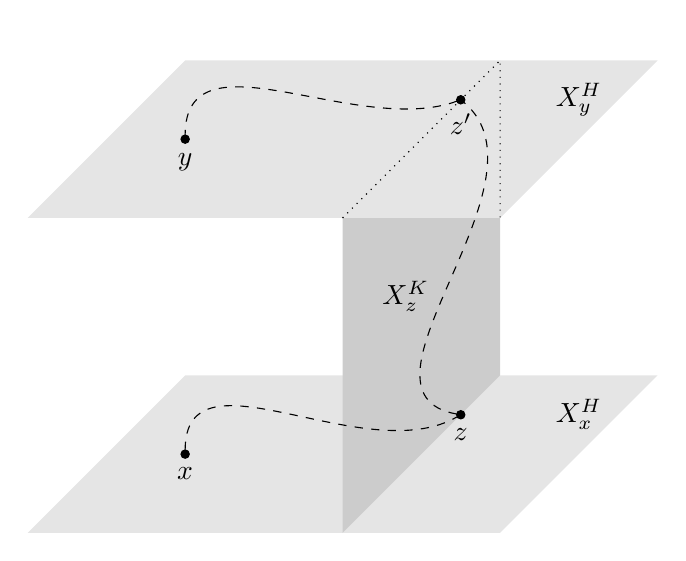
\begin{tikzpicture}
\fill[color = gray!20] (-4,0) -- (2,0) --(4,2) -- (-2,2) --cycle;
\fill[color = gray!40] (0,0) -- (2,2) --(2,6) -- (0,4) --cycle;
\fill[color = gray!20] (-4,4) -- (2,4) --(4,6) -- (-2,6) --cycle;
\draw [dotted] (0,4) -- (2,6) --(2,4);
\draw (3,1.5) node {$X_x^H$};
\draw (0.8,3) node {$X_z^K$};
\draw (3,5.5) node {$X_y^H$};
\node[style=blacknode, label={below:$x$}] (x) at (-2,1) {};
\node[style=blacknode, label={below:$z$}]  (z) at (1.5,1.5) {};
\node[style=blacknode, label={below:$z'$}]  (z') at (1.5,5.5) {};
\node[style=blacknode, label={below:$y$}]  (y) at (-2,5) {};
\draw [dashed] (x) to [out=90,in=210] (z) to [out=170,in=-40] (z') to [out=200,in=90] (y) ;
\end{tikzpicture}}
\caption{The path between $x$ and $y$.}
\label{Figure:PathSemiDirect}
\end{figure}

The action of $G$ on $X$ being transitive, there exists an element $(n_0,h_0)$ of $N \rtimes H$ such that $(n_0,h_0).x = y$.
Since $K'$ is finite, the set $X_x^H\setminus K'$ is infinite.
Moreover, there is infinitely many $z$ in $X_x^H\setminus K'$ such that either $X_z^N$ is one-ended or $X_z^N$ does not intersect $K'$.
For such a $z$ there exists $h$ such that $(1,h).x=z$.
Now, the vertex $z'\coloneqq(hh_0^{-1}n_0,h).x$ is both equal to $(hh_0^{-1}.n_0,1)(1,h_0).x=(hh_0^{-1}.n_0,1).z$ and to $(1,hh_0^{-1})(n_0,h_0).x=(1,hh_0^{-1}).y$. That is, $z'$ is in $X_z^N\cap X_y^H$.
A simple computation show us that the map $z\mapsto z'$ is injective: $z_1'=z_2'$ if and only if $z_1=z_2$.
Since $K'$ is finite, there is only finitely many $z'$ in $K'$ and hence there is infinitely many $z\in X_x^H$ such that both $z$ and $z'$ are not in $K'$ and either $X_z^N$ is one-ended or $X_z^N$ does not intersect $K'$.

In order to finish the proof, observe that the three graphs $X_x^H$, $X_y^H$ and $X_z^N$ are all either one-ended or do not intersect $K'$.
Therefore, there is a path in $X_x^H\setminus K'$ from $x$ to $z$ as desired, and so on for the paths from $z$ to $z'$ and $z'$ to $y$.
We just have proved that for any finite $K$ the graph $X\setminus K$ has only one infinite connected component and therefore that $X$ is one-ended.
%
%
%
%
%We claim that there exists a vertex $z$ of $X_x^H$ such that $X_z^N$ does not contain an element of $K'$ or is one-ended and such that $z'=(h'h^{-1}.n,0)z$ is not in $K'$, where $h'$ is an element of $H$ and $h'.x = z$. Indeed, such an element exists as $X_x^H$ and $X_y^H$ are infinite and $K$ is finite. The vertex $z'$ is in $X_y^H$ because
%\[
%(0,hh'^{-1}) z' = (0,hh'^{-1})(h'h^{-1}.n,0)(0,h')x = (n,h)x = y.
%\]
%
%We will construct a path on $X \setminus K$ between $x$ and $y$ as follows. The subgraph $X_x^H$ is one-ended, then there exists a path between $x$ and $z$. In the same way, $X_z^N$ has one end or has no vertex in $K$, then there is a path which join $z$ and $z'$. There exists a path between $z'$ and $y$ in $X_y^H$ which is one-ended. Then $x$ and $y$ are path-connected and then $X$ has one end. We proved that all the Schreier graph of $G$
\end{proof}
%geo

By iterating the last lemma, we obtain
%
%
\begin{cor}\label{Cor:Wreath_ends}
Let $G$ and $H$ be two finitely generated groups and $X$ a $H$-set such that the number of orbits is finite. Then,
\begin{enumerate}
\item
If $G\wr_X H$ has property FW, then so does $H$,
\item
If both $G$ and $H$ have property FW and $X$ is finite, then $G\wr_X H$ has property~FW.
\end{enumerate}
\end{cor}
%
%

%
%
\begin{lem}\label{Lem:Wreath_groups_ends}
Let $G$ and $H$ be two finitely generated groups such that $G\neq \{1\}$ and $H$ acts on some set $X$ with finitely many orbits.
If $G\wr_XH$ has property FW, then 
\begin{enumerate}
\item $G$ has property FW,
\item $X$ is finite.
\end{enumerate}
%
\begin{proof}
We will prove the contrapositives. The idea is to construct, for each of the two cases, a Schreier graph of $G\wr_XH$ with more than one end by exhibiting some well-chosen action of $G\wr_XH$.
We fix some finite generating sets $S$ and $T$ of $G$ and $H$ and let 
\[U\coloneqq\setst{(\delta_x^s,1_H)}{s \in S} \cup \setst{(\mathbf 1,t}{t \in T}\]
be the standard generating set of $G\wr_XH$.
%We will suppose, as in  Lemma~\ref{Lemma:Semidirect_ends} that $G = \gen{S}$ and $H = \gen{T}$ and $G_.

\paragraph{Suppose that $X$ is an infinite set.}
Since $H$ acts on $X$ with finitely many orbits, there exists an infinite orbit $X'$.
Let $x_0$ be an arbitrary vertex of $X'$.
%Let $x_0$ be an arbitrary vertex of $X'$ and let $Y$ be the set $Y = G \times X'$. The group $G\wr_XH$ acts on $Y$ via
The group $G$ acting on itself by left multiplications, we have the so-called \emph{imprimitive action} of the wreath-product $G\wr_XH$ on $Y\coloneqq G\times X'$:
\[
(\varphi,h). (g,x) \coloneqq (\varphi(h.x)g, h.x).
\]
Since both $G\curvearrowright G$ and $H\curvearrowright X'$ are transitive, the action $G\wr_XH\curvearrowright Y$ is also transitive. 
%The action is transitive. Indeed, let $(g_1,x_1)$ and $(g_2,x_2)$ be two elements of $Y$. By transitivity of the action of $H$ on $X'$, there exists $h$ in $H$ such that $hx_1 = x_2$ and $\varphi$ in $\bigoplus_X G$ such that $\varphi(hx_1) = g_2g_1^{-1}$. Then, 
%\[
%(\varphi,h) (g_1,x_1) = (\varphi(h x_1) g, h x_1) = (g_2,x_2).
%\]
Therefore, the orbital Schreier graph of $G\wr_XH\curvearrowright Y$ is isomorphic to the Schreier graph $\Gamma\coloneqq\Sch(G\wr_XH, \stab(1_G,x_0), U)$. We decompose this graph into leaves of the form $Y_g = \{ g \} \times X'$. There are two types of edges in $\Gamma$, which are coming from the two sets of generators, see Figure~\ref{Figure:Leaves}. The first ones, of the form $(\mathbf 1,t)$, give us on each leaf a copy of the orbital Schreier graph of $H \curvearrowright X'$. Indeed,
\[
(\mathbf 1,t).(g,x) = (g, t.x).
\]
The second ones, of the form $(\delta_{x_0}^s,1)$, give us loops everywhere except on vertices of the form $(g,x_0)$. By direct computation, we see that the vertices $(g,x_0)$ and $(sg,x_0)$ connect the leaves $Y_g$ and $Y_{sg}$, 
\[
(\delta_{x_0}^s,1)(g,x) = 
\begin{cases}
(g,x) & \textnormal{if }x \neq x_0, \\
(sg, x) & \textnormal{if }x = x_0.
\end{cases}
\]
%
\begin{figure}[htbp]\centering
\scalebox{0.7}{
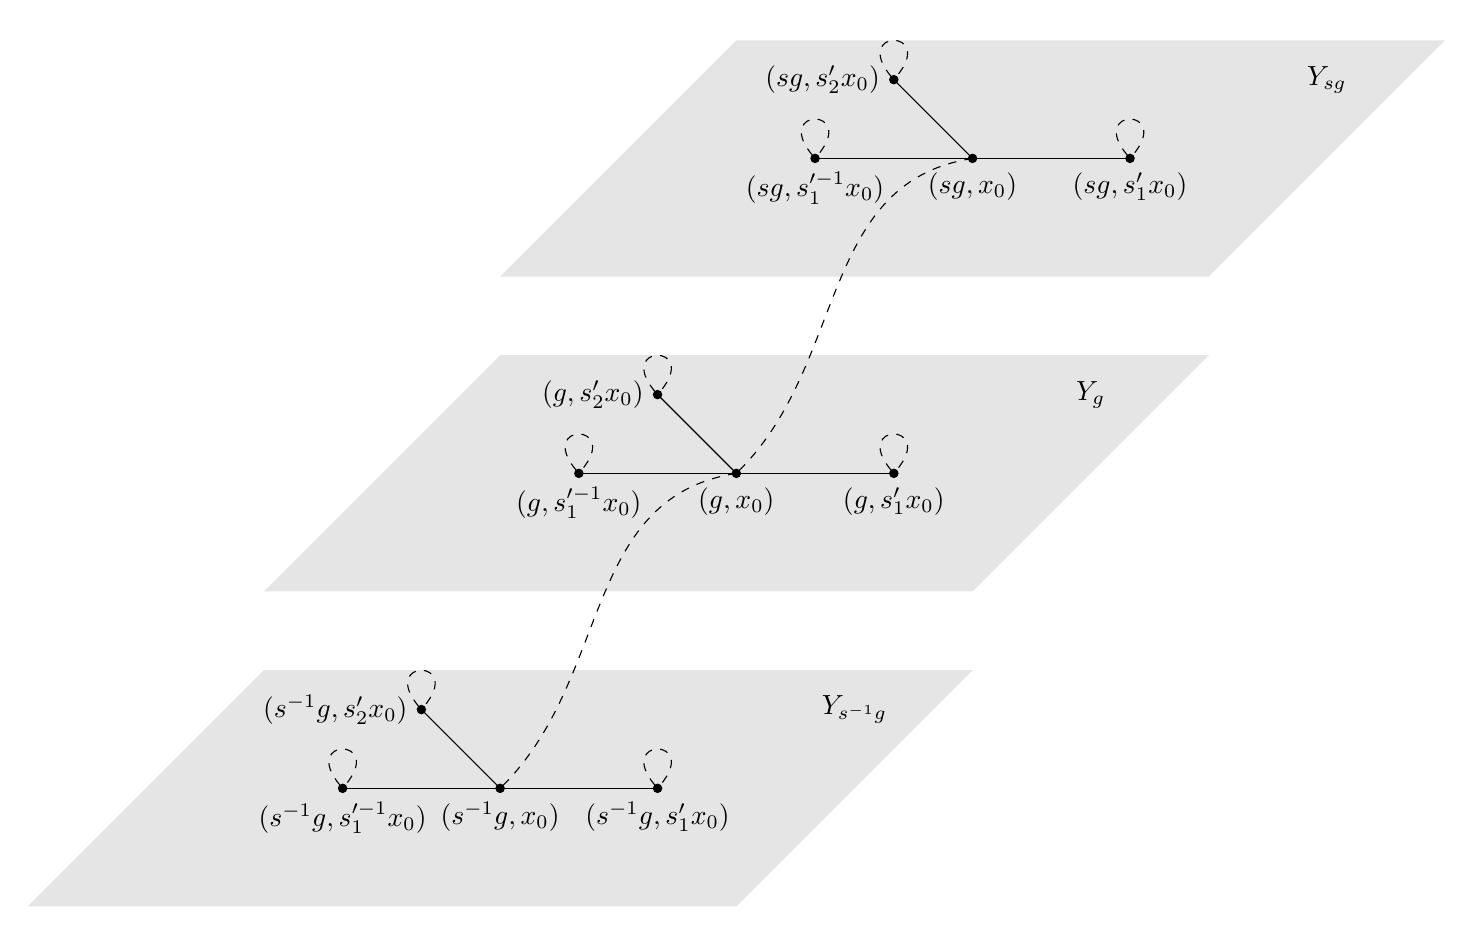
\begin{tikzpicture}
\fill[color = gray!20] (-6,-1.5) -- (3,-1.5) --(6,1.5) -- (-3,1.5) --cycle;
\draw (4.5,1) node {$Y_g$};
\node[style=blacknode, label= {below:$(g,x_0)$}] (00) at (0,0) {};
\node[style=blacknode, label={below:$(g,s'_1x_0)$}] (10) at (2,0) {};
\node[style=blacknode, label={below:$(g,s'^{-1}_1x_0)$}] (-10) at (-2,0) {};
\node[style=blacknode, label={left:$(g,s'_2x_0)$}] (20) at (-1,1) {};
\draw(-10) -- (00) -- (10);
\draw (20) -- (00);

\begin{scope}[shift = {(3,4)}]
\fill[color = gray!20] (-6,-1.5) -- (3,-1.5) --(6,1.5) -- (-3,1.5) --cycle;
\draw (4.5,1) node {$Y_{sg}$};
\node[style=blacknode, label={below:$(sg,x_0)$}] (01) at (0,0) {};
\node[style=blacknode, label={below:$(sg,s'_1x_0)$}] (11) at (2,0) {};
\node[style=blacknode, label={below:$(sg,s'^{-1}_1x_0)$}] (-11) at (-2,0) {};
\node[style=blacknode, label={left:$(sg,s'_2x_0)$}] (21) at (-1,1) {};
\draw(-11) -- (01) -- (11);
\draw (21) -- (01);
\end{scope}

\begin{scope}[shift = {(-3,-4)}]
\fill[color = gray!20] (-6,-1.5) -- (3,-1.5) --(6,1.5) -- (-3,1.5) --cycle;
\draw (4.5,1) node {$Y_{s^{-1}g}$};
\node[style=blacknode, label={below:$(s^{-1}g,x_0)$}] (02) at (0,0) {};
\node[style=blacknode, label={below:$(s^{-1}g,s'_1x_0)$}] (12) at (2,0) {};
\node[style=blacknode, label={below:$(s^{-1}g,s'^{-1}_1x_0)$}] (-12) at (-2,0) {};
\node[style=blacknode, label={left:$(s^{-1}g,s'_2x_0)$}] (22) at (-1,1) {};
\draw(-12) -- (02) -- (12);
\draw (22) -- (02);\end{scope}
\draw [dashed] (02) to [out=45,in=190] (00) to [out=45,in=190] (01);
\draw [dashed] (10) to [myloop above] (10) ;
\draw [dashed] (20) to [myloop above] (20) ;
\draw [dashed] (-10) to [myloop above] (-10) ;
\draw [dashed] (11) to [myloop above] (11) ;
\draw [dashed] (21) to [myloop above] (21) ;
\draw [dashed] (-11) to [myloop above] (-11) ;
\draw [dashed] (12) to [myloop above] (12) ;
\draw [dashed] (22) to [myloop above] (22) ;
\draw [dashed] (-12) to [myloop above] (-12) ;
\end{tikzpicture}}
\caption{The leaf structure of the orbital Schreier graph of $G\wr_XH \curvearrowright Y$. Plain edges correspond to generators of the form $(\mathbf 1,t)$ while dotted edges correspond to generators of the form $(\delta_{x_0}^s,1)$.}
\label{Figure:Leaves}
\end{figure}
%
If we remove a vertex $(g,x_0)$ we disconnect the leaf $Y_g$ from the rest of $\Gamma$. As $X'$ is infinite each leave is infinite and the number of ends of $\Gamma$ is then at least $\abs{G}\geq 2$. We just proved that if $X$ is infinite the group $G\wr_XH$ does not have property FW.

\paragraph{Suppose now that $G$ does not have property FW.} There exists a subgroup $K$ of $G$ such that $\Sch(G,K,S)$ has more than one end.
Let $x_0$ be any point of $X$ and $X'$ be its orbit under the action of $H$.
%The choice of $x_0$ is arbitrary in this case.
We have the imprimitive action of $G\wr_XH$ on $G/K\times X$, which we could restrict to an action on $G/K\times X'$:
\[
(\varphi,h)(gK,x) = (\varphi(h.x) gK, h.x).
\]
As above, the action is transitive and the orbital Schreier graph of this action is isomorphic to a Schreier graph $\Gamma$. We decompose this graph into leaves in the same way. Now we look at the subgraph made up of vertices $(g,x_0)$ and edges $(\delta_{x_0}^s,1)$ and we remark that it is isomorphic to the Schreier graph $\Sch(G,K,S)$ which has more than one end. Then $\Gamma$ has also more than one end, which finishes the proof.
\end{proof}
\end{lem}
%
%
The following proposition is a direct application of Corollary \ref{Cor:Wreath_ends} and Lemma \ref{Lem:Wreath_groups_ends}.
%
%
\begin{prop}
Let $G$ be a non trivial finitely generated group, $H$ be a finitely generated group and $X$ a set on which $H$ acts with a finite number of orbit. The wreath product $G \wr_X H$ has property FW if and only if $G$ and $H$ have property FW and $X$ is finite.
\end{prop}
%
%
\bibliography{biblio.bib}
\bibliographystyle{abbrv}











\enddocument